\section{Заключение}
	В данной работе были получены следующие основные результаты:
	\begin{itemize}
		\item Разработан метод, предсказывающий слабую масштабируемость суперкомпьютерных приложений на основе экспериментальных данных.
		\item Выполнена проверка применимости метода на различных приложениях, с помощью запусков приложений HPL, HPCG, матричных алгоритмов умножения SUMMA и DNS, Graph500 на суперкомпьютере "<Ломоносов-2">.
	\end{itemize}

	\begin{figure}
		\centering
		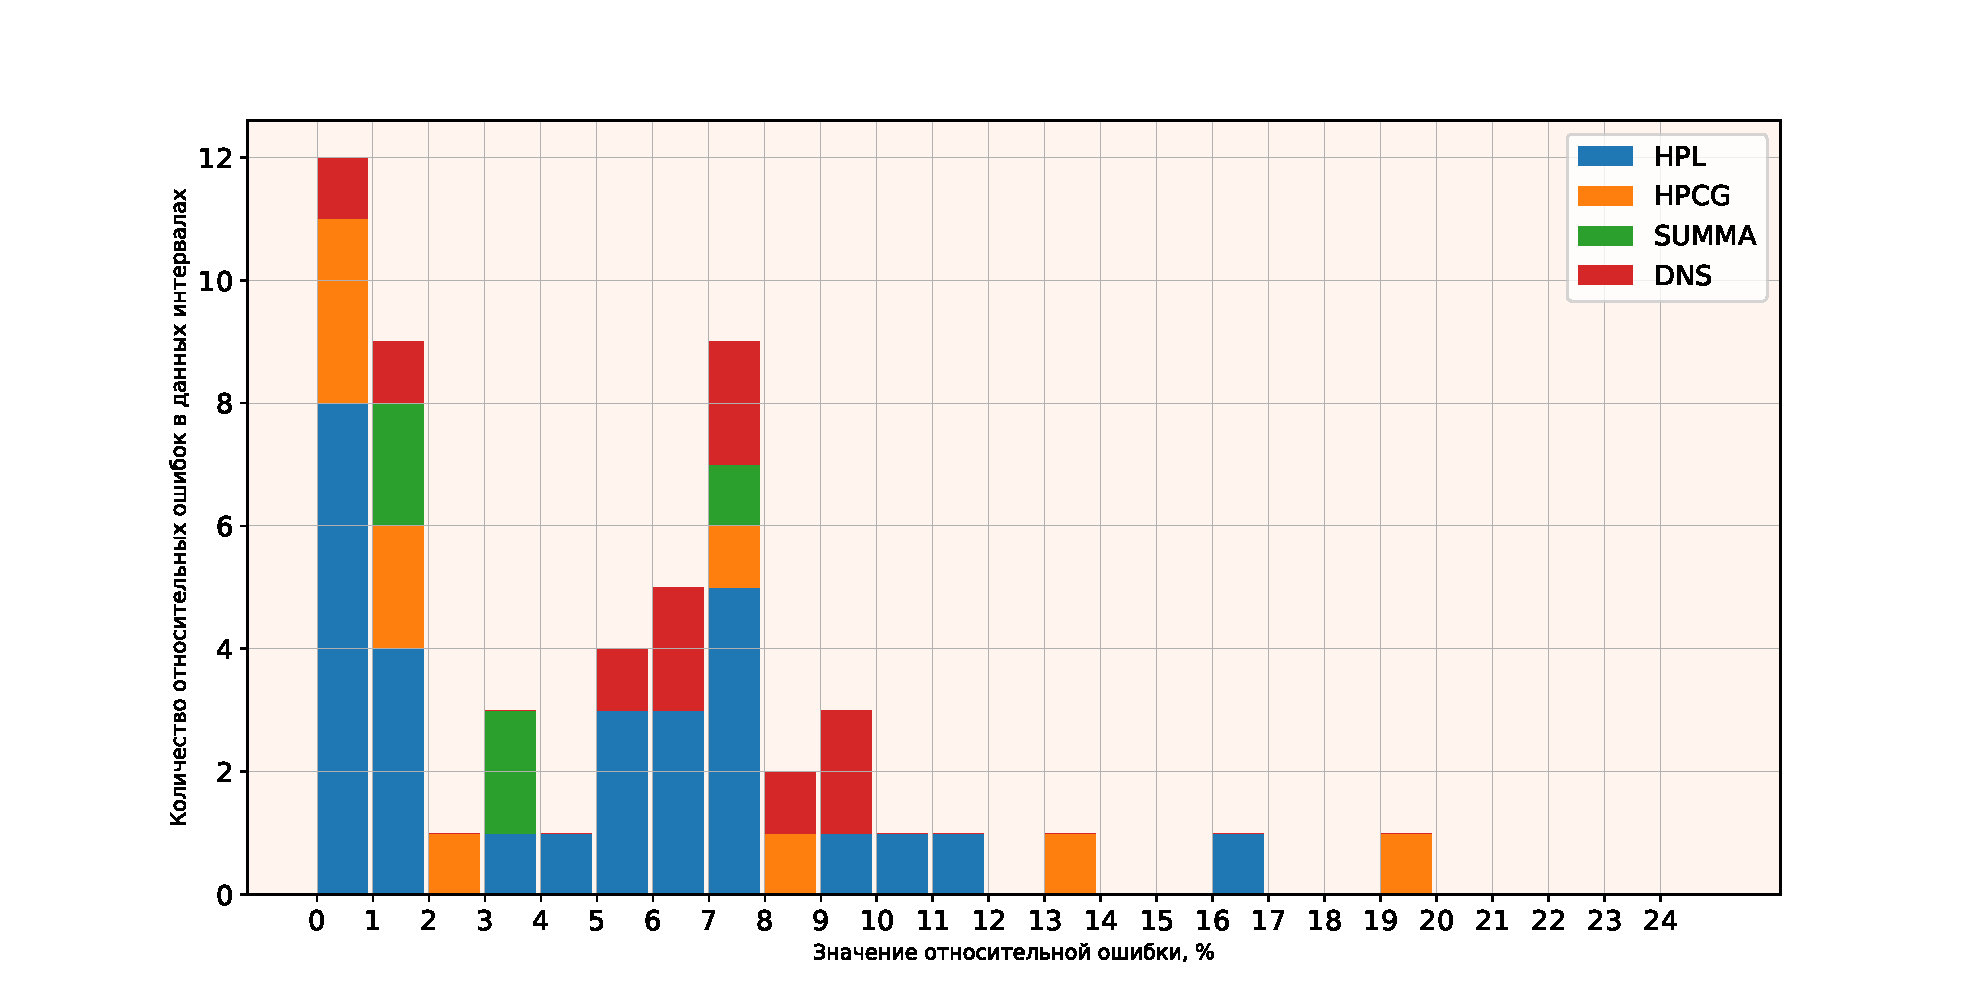
\includegraphics[width=\textwidth]{./images/conclusion_graph}
		\caption{Относительные ошибки предсказаний по всем рассматриваемым приложениям}
		\label{RESULT}
	\end{figure}

	На основании предложенного метода удалось построить предсказания слабой масштабируемости для всех рассматриваемых приложений так, что максимальная относительная ошибка среди всех приложений и конфигураций не превышает ???\%, а среднее значение относительной ошибки равно ???\%. Гистограмма с различными значениями относительных ошибок представлена на рисунке \eqref{RESULT}. Таким образом, предложенный метод предсказания даёт относительные ошибки, сравнимые с ошибками предсказания у существующих подходов при сопоставимых размерах конфигураций предсказываемых запусков. Но отличается от них простотой построения, отсутствием необходимости собирать большой набор тестовых данных. Помимо этого он удовлетворяет поставленным условиям универсальности.
\clearpage
%\newpage